\documentclass{llncs}

\usepackage{amsmath}
\usepackage{amssymb}
\usepackage{amsfonts}

\usepackage{bbm}
\usepackage{enumerate}

%\usepackage{fixme}
%\pagestyle{plain}


\usepackage{color}
\usepackage{cite}
\usepackage{graphicx}
\usepackage{pstricks}
\usepackage{amssymb}
\usepackage{amsfonts}
\usepackage{amsmath}
\usepackage[amsmath,thmmarks]{ntheorem}
\usepackage{todonotes}

\definecolor{mygreen}{rgb}{.0,.8,.0}
\newcommand{\greentext}[1]{\textcolor{mygreen}{#1}}


\begin{document}

\title{Similarity of medical imaging datasets}

%\author{*** \\ ***}
%\institute{* \\ * \\ * \\ *}

\author{Veronika Cheplygina\inst{1}, Pim Moeskops\inst{1}, Mitko Veta\inst{1}, Behdad Dashtbozorg\inst{1}, Josien P.W. Pluim\inst{1,2}}
% index{Cheplygina, Veronika} 
% index{Moeskops, Pim} 
% index{Veta, Mitko} 
% index{Dashtbozorg, Behdad} 
% index{Pluim, Josien} 

\institute{IMAG/e, Department Biomedical Engineering, Eindhoven University of Technology
\and Image Sciences Institute, University Medical Center Utrecht
}

%https://github.com/tueimage/bmpv

\maketitle

%1.     Abstract title
%2.     Author listing (all authors, principal author first), postal address, telephone, e-mail address.
%3.     Key words, list a maximum of five key words.
%4.     Abstract text providing information about:
%o    Purpose
%o    Methods
%o    Results
%o    References

\noindent \textbf{Keywords} machine learning, medical imaging, similarity, meta-learning

\section{Purpose}

Imagine you have experience with classification problems A and B and a colleague asks you for advice about problem C. Your advice will depend on your perceived similarity of problem C with A and B. This is called \emph{meta-learning} - predicting which methods will perform well in an unseen classification problem, based on previous experience. In this study, published in \cite{cheplygina2017exploring}, we investigate the first step: how to quantify the similarity of classification problems.

%What is the problem?
Our goal is to characterize the datasets in a meta-feature space, based on performances of simple classifiers. Dataset similarity is then defined to be inversely proportional to the Euclidean distances within this space. The best method for problem C can be decided based on whether A or B are closer. We present a toy experiment, where we investigate whether we can find a meaningful meta-feature space for this task. 

%Our aim is also to draw attention to meta-learning and highlight its potential value for medical image analysis. 
  


\section{Methods}\label{sec:methods} 

We start with datasets $\{(D_i, M_i)\}_{1}^{n}$, where $D_i$ is a dataset from a classification problem, like "tissue segmentation in brain MR". We use six classification problems, and sample from each problem 20 times, so $n=120$. $M_i$ is a meta-label, for example, the best classifier. For the toy experiment, we define $M_i$ as the original classification problem of $D_i$. 

\begin{figure}
\centering
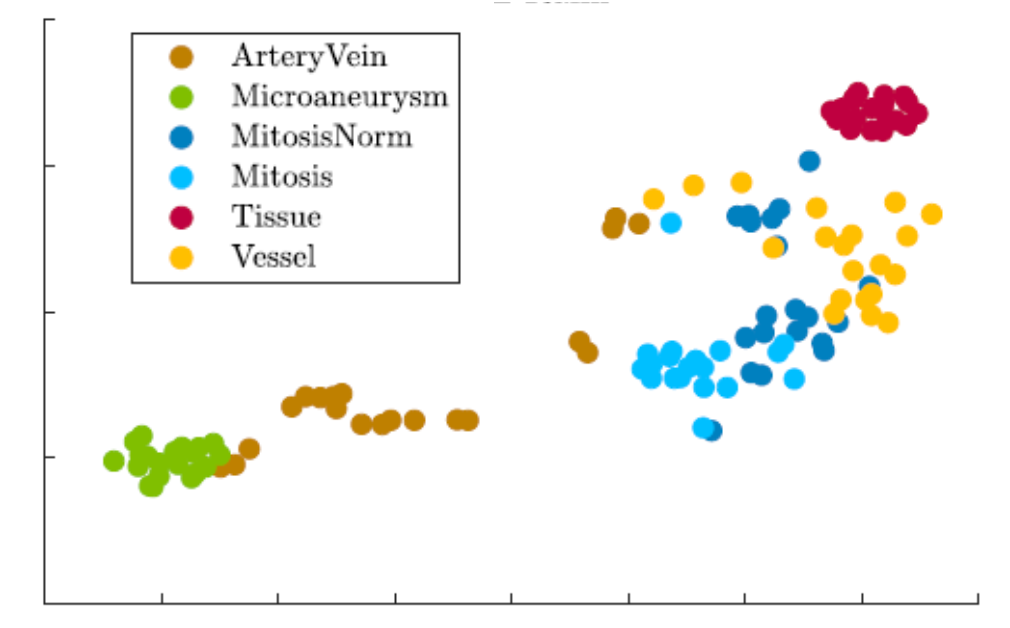
\includegraphics[width=0.75\textwidth]{tsne_rank.png}%
\caption{(t-SNE embedding of ranks of six simple classifiers, for 120 datasets from six different classification problems.}
\label{fig:overview}
\end{figure}

We represent each dataset by normalized accuracies (for fair comparisons) of $k$ simple classifiers, like nearest neighbor and decision trees.  Together these representations form a $n \times k$ meta-dataset $N_k$. We then embed this meta-datasets with  multi-dimensional scaling (MDS) and t-stochastic nearest neighbor embedding (t-SNE). 






\section{Results}\label{sec:results}

An example of an embedding is shown in Fig.~\ref{fig:overview}. In some cases, datasets we expect to be similar are in fact similar. For example ArteryVein and Microaneurysm both use retinal images, and Mitosis and MitosisNorm datasets use the same images but with different normalization. The Tissue dataset is the most different from the rest, being the only dataset based on 3D MR images. Other similarities cannot be explained. We would expect Vessel to be similar to ArteryVein and Microaneurysm, but it is actually more similar to Mitosis and MitosisNorm. 

When this embedding is used for classification (predicting what dataset it is, based on normalized accuracies), we can achieve an error of 10.7\%, when training on 60 datasets, and testing on the other 60. This is reasonable for a six-class problem classification problem. 

This is a toy experiment, because we use artifical meta-labels. However, we would not expect the best-performing classifier to change, if we have a different sampling from the same classification problem. Validating the approach with classifier-based meta-labels is the next step for a more practical application of this method. Other directions include investigating different feature extraction methods (now the features were fixed for each problem) and taking human similarity judgments into account.



\bibliographystyle{splncs}
\bibliography{refs}

\end{document}